\documentclass{article}
\usepackage{tikz}
\usepackage{pgfplots}
\usepackage{svg}
\usepackage{amsmath}
\usepackage{array}
\usepackage[skins]{tcolorbox}
\usepackage[version=4]{mhchem}
\usepackage[a4paper, total={6in, 9in}]{geometry}
\usepackage{fourier}
\usepackage{xymtex}
\usepackage{textcomp}
\usepackage{eurosym}
\usepackage{caption}
\usepackage{longtable}
\usepackage{float}
\usepackage{attachfile}
\usepackage{multirow}
\usepackage{amsfonts} 
\usepackage{tabularray}
\usepackage{colortbl}
\usepackage{xcolor}
\usepackage{graphicx}
\usepackage[table]{xcolor}
\UseTblrLibrary{booktabs}
\usepackage[bottom]{footmisc}

\captionsetup[table]{name=Tabella}
%<\pagenumbering{gobble}


\renewcommand*\contentsname{Indice}
\setcounter{tocdepth}{3}
%\setcounter{secnumdepth}{2}
\pgfplotsset{compat=1.15}


\title{Relazione di laboratorio - Periodo di un pendolo semplice}
\author{Federico Cesari}
\date{Aprile 2024}





%%%%%%%%%%%%%%%%%%%%%%%%%%%%%%%%%%%%%%%%%%%%%%%%%%%%%%%%%
%%				INIZIO DOC
%%%%%%%%%%%%%%%%%%%%%%%%%%%%%%%%%%%%%%%%%%%%%%%%%%%%%%%%%


\begin{document}
	\begin{titlepage}
	\begin{center}
		\vspace*{1cm}
		
		\textbf{\LARGE Relazione di laboratorio - Pendolo semplice}
		
		\vspace{0.3cm}
		\large \textit{Misura del periodo di un pendolo semplice} \\
		
		\vspace{0.5cm}
		\Large Federico Cesari \\
		
		\small 1096759 
		\vspace{0.2cm}
		
		\small Gruppo 5
		
		
		\vspace{3cm}
		\begin{center}
			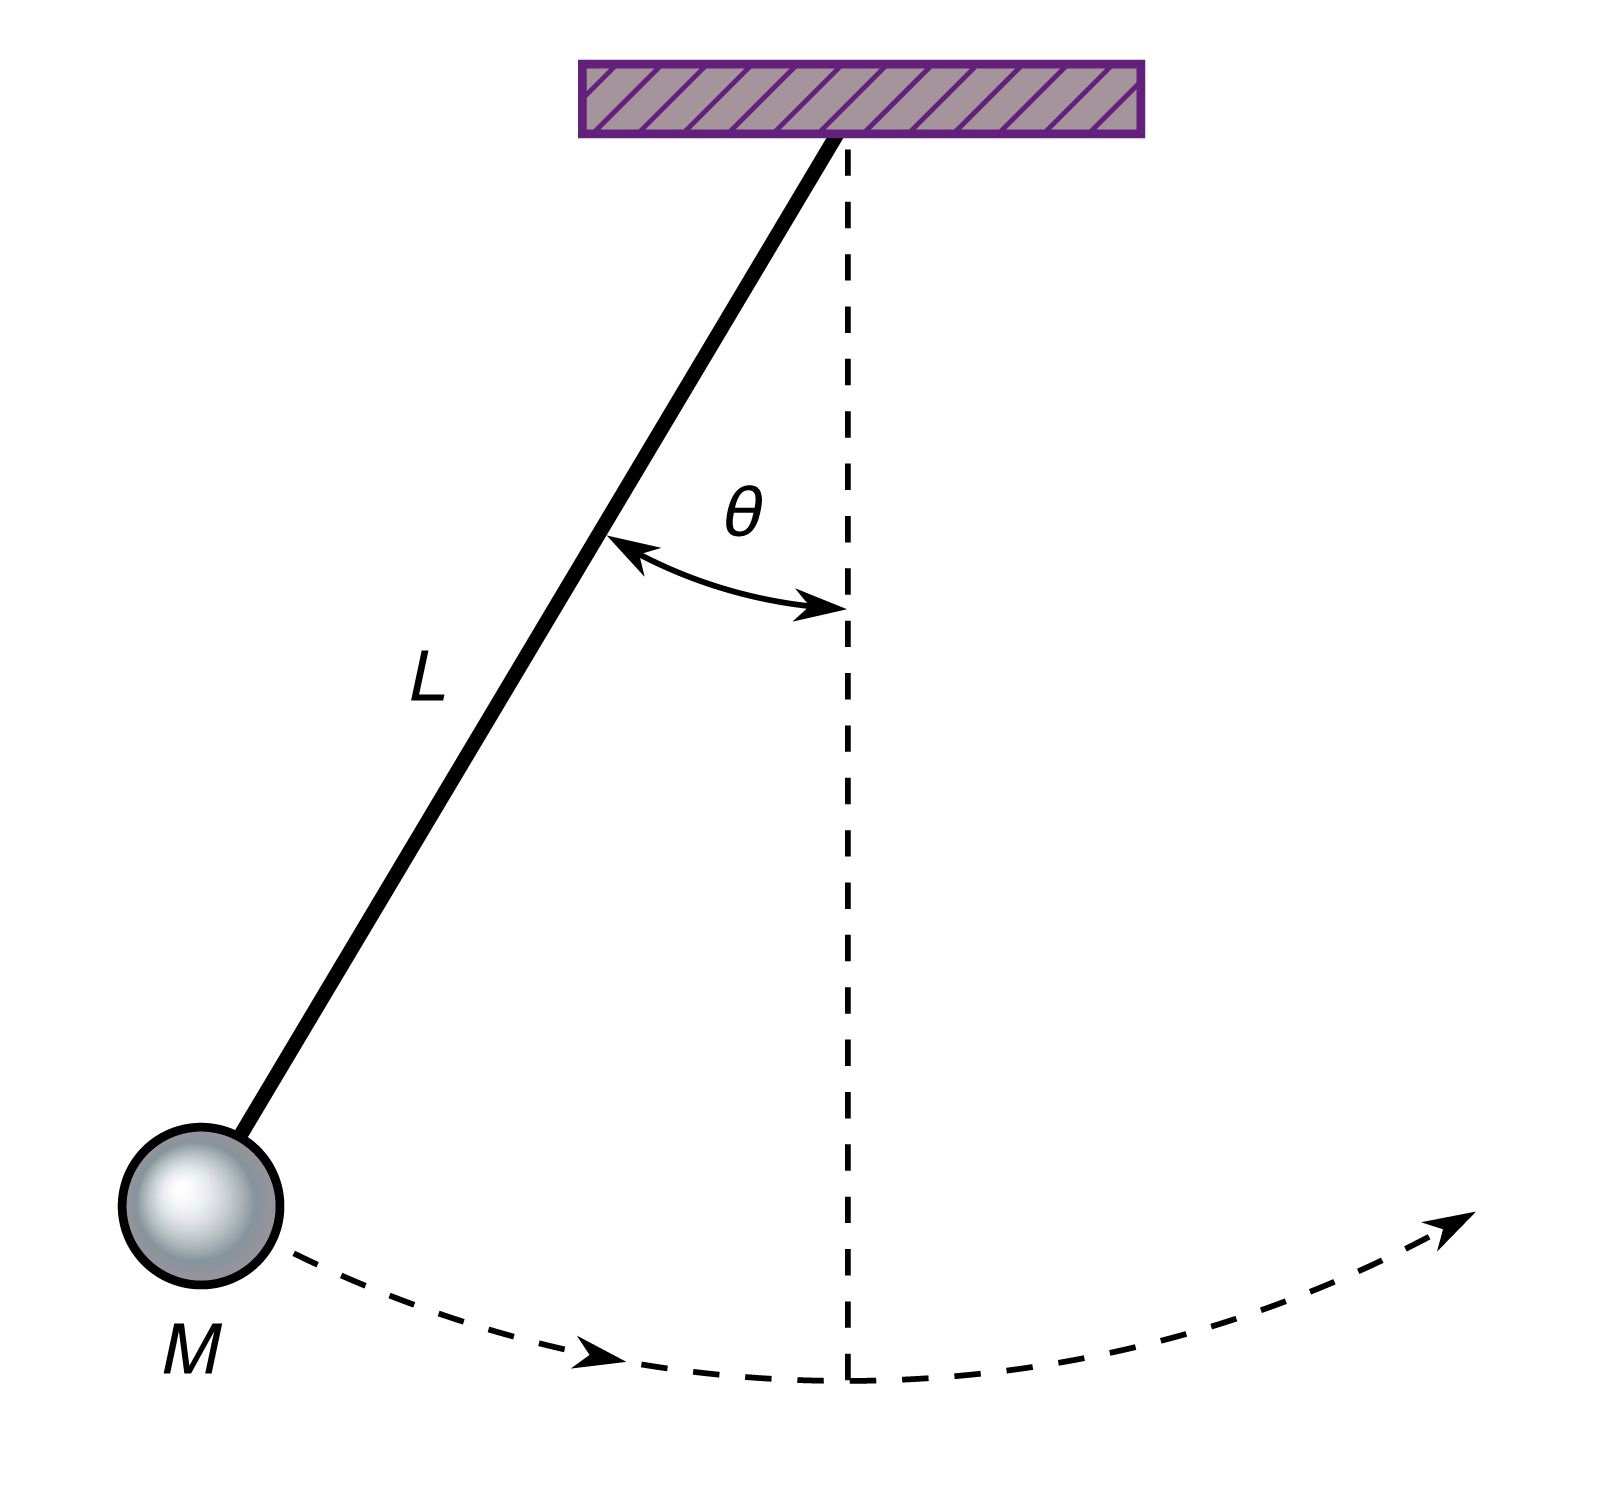
\includegraphics[scale=0.1]{IMG_0200.jpeg}	
		\end{center}
		
		
		
		\vfill
		
		
		
		corso A\\
		Università degli studi di Torino, Torino\\
		4 aprile 2024\\
		
		
	\end{center}
\end{titlepage}
	\tableofcontents
	
	\newpage
	\textcolor{white}{.}
	\vfill
	\section{Scopo dell’esperienza}
	L'esperienza di laboratorio ha lo scopo di studiare il periodo di un pendolo semplice del quale sono note le espressioni del periodo teorico (in condizioni ideali e prive di attrito) in funzione della sua lunghezza e dell'angolo di oscillazione. Verrà quindi misurato il periodo e se ne osserverà la dipendenza dall'angolo, dalla lunghezza e dalla massa appesa ad esso.
	
	\paragraph{Aspettative} Dall'equazione teorica del periodo del pendolo 
	\begin{equation} \label{eq:1}
		T = T_0\left[1 + \frac{1}{4}\sin{(\vartheta/2)^2}\right] \qquad  T_0 = 2\pi \sqrt{\frac{l}{g}} 
	\end{equation}
	si evince che per angoli maggiori di $10^\circ$ il periodo dipende dalla lunghezza $l$ del pendolo e dall'angolo di oscillazione $\vartheta$, mentre per angoli più piccoli di  $10^\circ$ l'angolo di partenza incide sempre di meno diventando trascurabile. Non dipende invece dalla massa.
	
	\section{Strumentazione}
	La strumentazione utilizzata durante l'esperienza è:
	
	\begin{table}[H]
		\centering
		\begin{tabular}{@{}ll@{}}
			\textbf{Strumento} & \textbf{Sensibilità} \\ \midrule
			Cronometro Analogico      & $0.2$s               \\
			Cronometro Digitale       & $0.01$s              \\
			Fotocellula        & $0.001$s             \\
			Goniometro         & $1^\circ$            \\
			Asta graduata      & $0.1$cm              \\
			Calibro            & $0.01$mm             \\
			Bilancia digitale  & $1$g                 \\ \bottomrule
		\end{tabular}
	\end{table}
	\noindent
	In più sono servite alcune sfere di diversi materiali e naturalmente un pendolo semplice di lunghezza variabile.
	
	Tutti gli angoli di partenza saranno misurati con il goniometro, le masse delle sfere con la bilancia digitale e la lunghezza del pendolo con l'asta graduata. I periodi di oscillazione saranno acquisiti con la fotocellula (preferita ai due cronometri per le conclusioni tratte nel punto successivo).
	

	
	%%%%%%%%%%%%%%%%%%%%%%%%%%%%%%%%%%%%%%%%%%%%%%%%%%%%%%%%%
	%%				SCELTA STRUMENTO
	%%%%%%%%%%%%%%%%%%%%%%%%%%%%%%%%%%%%%%%%%%%%%%%%%%%%%%%%%
	
	
	
	\newpage
	\section{Scelta strumento di misura}
	
	Al fine di stabilire il migliore strumento di misura per le succesive misurazioni, registro 8 misure del periodo del pendolo prima con un angolo di partenza $\vartheta = 5^\circ \pm1^\circ$ e poi con $\vartheta = 30^\circ\pm1^\circ$, utilizzando un cronometro analogico, uno digitale e una fotocellula. Lo strumento che mostrerà discrepanze significative tra il periodo calcolato con $\vartheta = 5^\circ\pm1^\circ$ e $\vartheta = 30^\circ\pm1^\circ$ sarà quello utilizzato per nelle acquisizioni successive. Procedo quindi con le misurazioni dei periodi del pendolo a cui è stata agganciata una sfera di massa $m = (110 \pm 1)g$ evidenziando il periodo medio $\mathbf{\bar{T}(s)}$ e la deviazione standard $\sigma_{T_{5}}$ delle 8 misure. 
	
	\vspace{1cm}
	\begin{minipage}{0.5\textwidth}
		\begin{table}[H]
			\hspace{-1.7cm}
			\begin{tabular}{@{}lrrr@{}}
				&\textbf{C.Analogico} & \textbf{C. Digitale} & \textbf{Fotocellula} \\ \cmidrule(l){2-4} &\multicolumn{1}{l}{$T(s) \pm 0.2s$} & \multicolumn{1}{l}{$T(s) \pm 0.01s$}   & \multicolumn{1}{l}{$T(s) \pm 0.001s$}    \\ \cmidrule(l){2-4} 
				
				\multicolumn{1}{c}{}  
				& 1.6   & 1.63   & 1.702     \\
				\colorbox{orange!40}{$\vartheta = 5^\circ$}   & 1.8   & 1.65   & 1.703     \\
				\multicolumn{1}{r}{\colorbox{orange!40}{$\pm 1^\circ$}}& 1.5   & 1.60   & 1.703     \\ 
				& 1.8   & 1.71   & 1.703     \\
				& 1.7   & 1.71   & 1.703     \\
				& 1.5   & 1.65   & 1.702     \\
				& 1.6   & 1.70   & 1.703     \\
				& 1.5   & 1.70   & 1.703     \\ \arrayrulecolor{black!100}\specialrule{1.2pt}{0.5\jot}{0.5pc}
				
				$\mathbf{\bar{T}_{5}(s)}$  & \textbf{1.6}    & \textbf{1.67}  & \textbf{1.703}  \\
				$\sigma_{T_{5}}$(s)  & 0.05    & 0.02  & 0.000 \\                          
			\end{tabular}
		\end{table}
	\end{minipage}
	\begin{minipage}{0.5\textwidth}
		\begin{table}[H]
			\centering
			\begin{tabular}{@{}lrrr@{}}
				&\textbf{C.Analogico} & \textbf{C. Digitale} & \textbf{Fotocellula} \\ \cmidrule(l){2-4} &\multicolumn{1}{l}{$T(s) \pm 0.2s$} & \multicolumn{1}{l}{$T(s) \pm 0.01s$}   & \multicolumn{1}{l}{$T(s) \pm 0.001s$}    \\ \cmidrule(l){2-4} 
				
				\multicolumn{1}{c}{}  
				& 1.8   & 1.65   & 1.733     \\
				\colorbox{blue!40}{$\vartheta = 30^\circ$}  & 1.7   & 1.67   & 1.733     \\
				\multicolumn{1}{r}{\colorbox{blue!40}{$\pm 1^\circ$}} & 1.6   & 1.70   & 1.733     \\ 
				& 1.7   & 1.62   & 1.733     \\
				
				& 1.7   & 1.70   & 1.731     \\
				& 1.8   & 1.72   & 1.733     \\
				& 1.7   & 1.80   & 1.733     \\
				& 1.6   & 1.69   & 1.732     \\ \arrayrulecolor{black!100}\specialrule{1.2pt}{0.5\jot}{0.5pc}
				
				$\mathbf{\bar{T}_{30}(s)}$ & \textbf{1.7}    & \textbf{1.69}  & \textbf{1.715}  \\
				$\sigma_ {T_{30}}$(s)   & 0.08    & 0.03  & 0.0005 \\                          
			\end{tabular}
		\end{table}
	\end{minipage}
	\vspace{1cm}
	
	\noindent
	Da questi primi set di dati noto subito che la deviazione standard dei periodi misurati dal cronometro digitale è più grande della sensibilità dello strumento, scelgo quindi la deviazione standard come incertezza sulla singola misura.
	
	
	Per i test successivi sarà necessario che lo strumento di misura dei periodi di oscillazione distingua periodi differenti per angoli differenti, quindi, per evidenziare quale dei tre strumenti fornisca periodi significativamente distinguibili per i due angoli di partenza, sottopongo le coppie di periodi medi a due test Z (utilizzando in uno $\sigma_{\bar{T}_5}$ e nell'altro $\sigma_{\bar{T}_30}$) per verificarne la compatibilità:
	
	\paragraph{Ipotesi nulla} I periodi di oscillazioni acquisiti per angoli di oscillazione di $\sigma_{\bar{T}_5}$ e $\sigma_{\bar{T}_30}$ con la fotocellula non sono compatibili.
	
	\begin{table}[H]
		\centering
		\begin{tabular}{@{}lrr@{}}
			\toprule
			Z & \multicolumn{1}{l}{$\sigma_{\bar{T}_5}$} & \multicolumn{1}{l}{$\sigma_{\bar{T}_{30}}$} \\ \midrule
			$z_{\text{an.}}$      & \textit{\textbf{0.234}}                  & \textit{\textbf{0.234}}                   \\
			$z_{\text{dig.}}$     & \textit{\textbf{0.170}}                  & \textit{\textbf{0.132}}                   \\
			$z_{\text{fot.}}$     & \textit{\textbf{22.8}}                   & \textit{\textbf{14.2}}                    \\ \bottomrule
		\end{tabular}
	\end{table}
	
	\paragraph{Conclusione test}
	Il test mostra che i periodi misurati con i cronometri analogico e digitale con angoli di partenza $\vartheta = 5^\circ$ e $\vartheta = 30^\circ$ ($\pm 1^\circ$) forniscono un valore di $z$ osservato minore di 0.2, perciò  risultano essere compatibili con livelli di significatività maggiori dell'80\%. Per quanto riguarda i periodi registrati con la fotocellula invece, risultano essere totalmente incompatibili con valori di $z$ osservato maggiori di 14; posso quindi affermare che lo strumento che rileva periodi significativamente differenti per i due angoli di partenza sia proprio la fotocellula.
	
	
	
	
	
	
	
	
	%%%%%%%%%%%%%%%%%%%%%%%%%%%%%%%%%%%%%%%%%%%%%%%%%%%%%%%%%
	%%				DIPENDENZA THETA   00000
	%%%%%%%%%%%%%%%%%%%%%%%%%%%%%%%%%%%%%%%%%%%%%%%%%%%%%%%%%
	
	\newpage
	\section{Dipendenza dall’angolo}
	La prima parte dell'esperienza consiste nel verificare la dipendenza di $T$, periodo del pendolo a cui è stata attaccata una sferetta di legno di massa $m = (10 \pm 1)g$, da $\vartheta$, angolo di oscillazione.  Per prima cosa si procede alla misurazione della lunghezza del pendolo:	con l'asta graduata misuro prima la distanza da terra alla cima del pendolo ($L_C$) e poi la distanza da terra al centro della sfera appesa ($L_F$)\footnote{Avrei potuto misurare il diametro della sfera con il calibro e aggiungere il raggio della sfera successivamente invece che includerlo nelle misura di cima e fondo, tuttavia la sensibilità dell'asta e il fatto che questa non fosse perfettamente perpendicolare al piano di lavoro ha reso gli errori di $L_C$ e $L_F$ troppo grossolani rendendo così inutile la maggiore cura nella misura del raggio.}.   \begin{equation}
		l = L_C - L_F 
	\end{equation} \label{eq:2}
	misuro $L_C = (89.0 \pm 0.1)$cm e $L_F = (16.8 \pm 0.1)$cm. 
	Ricavo quindi la lunghezza del pendolo:
	\[
	l = L_C - L_F = (72.2 \pm 0.2) \text{cm}. \footnote{Propago l'errore linearmente ($\left(0.1 + 0.1 \right)\text{cm} = 0.2\text{cm}$ perché essendo solo due misure (per di più effettuate con un asta graduata imperfetta) rischio di sottostimare l'errore sommandolo in quadratura}
	\] 
	
	\subsection{Acquisizione dati}
	
	A questo punto prendo tre misurazioni del periodo del pendolo per 6 angoli di partenza differenti. Con l'ausilio di un goniometro con sensibilità di $1^\circ$, partendo da un angolo di oscillazione di $5^\circ$, registro tre misure. Faccio lo stesso con  $\vartheta = 10^\circ$, $\vartheta = 15^\circ$  continuando con un passo di $5^\circ$ fino ad arrivare a un angolo di $30^\circ$. Finita la presa dati ottengo i seguenti periodi con i relativi  periodi medi:
	
	
	\vspace{0.7cm}
	\begin{minipage}{1\textwidth}
	\begin{table}[H]
		\centering
		\begin{tabular}{@{}lrrrrrr@{}}
			& $\mathbf{5^\circ}$ \footnote{tutti gli angoli di oscillazione hanno un'incertezza di $1^\circ$}& $\mathbf{10^\circ}$ & $\mathbf{15^\circ}$ & $\mathbf{20^\circ}$ & $\mathbf{25^\circ}$ & $\mathbf{30^\circ}$  \\ \cmidrule(l){2-7}   
			& $T(s) \pm 0.001s$ & $T(s) \pm 0.001s$   & $T(s) \pm 0.001s$ & $T(s) \pm 0.001s$ & $T(s) \pm 0.001s$ & $T(s) \pm 0.001s$  \\ \cmidrule(l){2-7} 
			
			\multicolumn{1}{c}{}  
			
			&1.703 & 1.706 & 1.710 & 1.715 & 1.723 & 1.730  \\
			&1.702 & 1.706 & 1.710 & 1.715 & 1.723 & 1.731 \\
			&1.701 & 1.706 & 1.710 & 1.715 & 1.723 & 1.731 \\
			
			\arrayrulecolor{black!100}\specialrule{1.2pt}{0.5\jot}{0.5pc}
			
			$\mathbf{\bar{T}(s)}$ \footnote{L'errore su $\bar{T}$ sarebbe minore della sensibilita ($0.001$s) quindi associo quest'ultima come incertezza sui valori calcolati }  & \textbf{1.702}    & \textbf{1.706}  & \textbf{1.710} & \textbf{1.715} & \textbf{1.723} &  \textbf{1.731}        
		\end{tabular}
	\end{table}
	\end{minipage}
	\vspace{1cm}
	
	\noindent
	Dall'espressione del periodo del pendolo sappiamo che il periodo è direttamente proporzionale a $\sin\left(\vartheta/2\right)^2$, più precisamente:
	\[
	T = T_0 \left[ 1 + \frac{1}{4}\sin{\left(\vartheta/2\right)}^2 \right]
	\]
	Se dovessi riportare su un grafico i periodi sperimentali $T(\bar{y})$ in funzione di $\bar{y} = \sin{\left(\vartheta/2\right)}^2$ mi aspetto un andamento lineare e più precisamente una retta del tipo
	
	\[
	T = T_0 + \frac{T_0}{4}\bar{y}
	\]

	
	\subsection{Retta di best-fit}
	Appurato che $T$ e $\sin{\left(\vartheta/2\right)}^2$ siano \textit{teoricamente} linearmente correlati, è di mio interesse trovare quale retta della forma $T = a + by$ meglio interpola i dati sperimentali così da appurare se i valori misurati soddisfano la attesa teorica che $y$ sia lineare in $x$. 
	
	Posso fare questo avvalendomi del metodo dei minimi quadrati che ha  proprio lo scopo di determinare i parametri che legano due variabili, nel mio caso due parametri $A$ e $B$ che legano due variabili $x$ e $y$. Questo metodo necessita di alcune assunzioni importanti: 
	
	\begin{enumerate}
		\item Le misure devono essere statisticamente indipendenti;
		\item Una delle due variabili (sceglierò la $x$) deve avere errori trascurabili rispetto all'altra; \footnote{Giudico un errore come trascurabile rispetto all'altro quando si trovano in rapporto 1 a 3,4,5...}
		\item Gli errori della variabile $y$ devono essere distribuiti normalmente.
	\end{enumerate}
	
	\noindent
	Per rispettare la seconda assunzione confronto gli errori relativi delle mie due variabili ($\sigma_x$ è l'errore assoluto, $\sigma_x/x$ è l'errore relativo).
	
	\begin{minipage}{0.5\textwidth}
		\begin{table}[H]
			\centering
			\begin{tabular}{@{}ccc@{}}
				\multicolumn{3}{c}{$\mathbf{T}$} \\ \midrule
				$T(s)$ & $\sigma_T (s)$ & $\sigma_T / T$ \\ \midrule
				1.702 & 0.001 & \textbf{0.00034} \\
				1.706 & 0.001 & \textbf{0.00034} \\
				1.710 & 0.001 & \textbf{0.00034} \\
				1.715 & 0.001 & \textbf{0.00034} \\
				1.723 & 0.001 & \textbf{0.00034} \\
				1.731 & 0.001 & \textbf{0.00033}  \\ \bottomrule   
			\end{tabular}
		\end{table}
	\end{minipage}
	\begin{minipage}{0.5\textwidth}
		\begin{table}[H]
			\centering
			\begin{tabular}{@{}ccc@{}}
				
				\multicolumn{3}{c}{$\bar{y} = \mathbf{sin{\left(\vartheta/2\right)}^2}$} \\ \midrule
				$\bar{y}$ & $\sigma_{\bar{y}}$ & $\sigma_{\bar{y}} / \bar{y}$ \\ \midrule
				0.002&0.001 & \textbf{0.40} \\
				0.008&0.002 & \textbf{0.20}  \\
				0.017&0.002 & \textbf{0.13}  \\ 
				0.030&0.003 & \textbf{0.01}  \\
				0.047&0.004 & \textbf{0.08}  \\
				0.067&0.004 & \textbf{0.07}  \\ \bottomrule  
			\end{tabular}
		\end{table}
	\end{minipage}
	\footnote{Lascio 3 cifre significative negli errori relativi del periodo per evidenziarne le piccole discrepanze.}
	\vspace{1cm}
	
	\noindent
	Come si può leggere nelle tabelle l'errore associato alle misure dei periodi è perfettamente trascurabile rispetto a quello associato al seno, quindi scelgo di portare le misure del periodo sull'asse $x$ e quelle del seno sull'asse $y$. \\
	
	\noindent
	La funzione da linearizzare non è più 
	\[
	T = a + b\bar{y}
	\]
	ma bensì
	\[
	\bar{y} = \mathbf{A} + \mathbf{B}T
	\]
	
	
	
	\begin{minipage}{0.3\textwidth}
		\begin{table}[H]
			\centering
			\begin{tabular}{@{}ll@{}}
				$T(s)$ & $\sin{\left(\vartheta/2\right)}^2 \pm \sigma_{\bar{y}}$ \\ \midrule
				1.702&0.002 $\pm 0.001$   \\
				1.706&0.008 $\pm 0.002$  \\
				1.710&0.017 $\pm 0.002$   \\
				1.715&0.030 $\pm 0.003$   \\
				1.723&0.047 $\pm 0.004$   \\
				1.731&0.067 $\pm 0.004$   \\	\bottomrule
			\end{tabular}
		\end{table}
		\[
		\mathbf{A} = -3.68 \qquad \mathbf{\sigma_A} = 0.18 
		\]
		\[ 
		\mathbf{B} = 2.16  \text{ (1/s)} \qquad \mathbf{\sigma_B} = 0.10  \text{ (1/s)}
		\]
	\end{minipage}
	\begin{minipage}{0.7\textwidth}
		\begin{figure}[H]
			\centering
			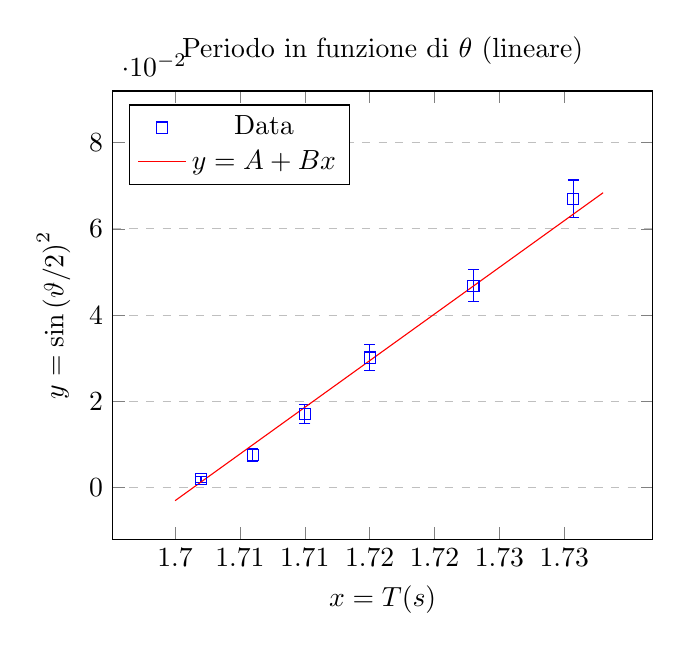
\begin{tikzpicture}
				\begin{axis}[
					title={Periodo in funzione di $\theta$ (lineare)},
					xlabel={$x = T(s)$},
					ylabel={$y = \sin{\left( \vartheta / 2\right) }^2$},
					xmin=1.7, xmax=1.732,
					ymin=0, ymax=0.08,
					xtick={1.7,1.705,1.71,1.715,1.72,1.725,1.73},
					ytick={0,0.02,0.04,0.06,0.08},
					legend pos=north west,
					ymajorgrids=true,
					grid style=dashed,
					enlargelimits=0.15,
					]
					
					\addplot[
					only marks,
					color=blue,
					mark=square,
					error bars/.cd,
					y dir=both, y explicit
					]
					coordinates {
						(1.702,0.0019027) +- (0,0.00075825)
						(1.706,0.0075961) +- (0,0.00151074)
						(1.710,0.0170371) +- (0,0.00225173)
						(1.715,0.0301537) +- (0,0.00297558)
						(1.723,0.0468461) +- (0,0.00367678)
						(1.7307,0.0669873) +- (0,0.00435)
					};
					\addplot[
					domain=1.7:1.733, 
					samples=100, 
					color=red, 
					] 
					{2.16490*x -3.68337};
					\legend{Data,$y=A+Bx$}
				\end{axis}
			\end{tikzpicture}
		\end{figure}
	\end{minipage}
	
	
	
	\subsubsection{Test del chi quadro}
	Visti i risultati ottenuti assumo che la retta trovata di parametri $\mathbf{A}$ e $\mathbf{B}$ si adatti bene all'andamento dei miei dati. Per assicurarmene effettuo un test del $\chi^2$.
	
	\paragraph{Ipotesi nulla} La retta $y = A + Bx$ descrive bene l'andamento dei dati osservati sperimentalmente.
	
	\vspace{0.7cm}
	\begin{table}[H]
		\centering
		\rowcolors{1}{gray!25}{white}
		\begin{tabular}{lr} 
			Livello di significatività $\alpha$		&$\quad 0.05$  \\
			Valore di $\chi ^2$             	& $\quad 4.29$       \\
			Numero di gradi di libertà      	& $\quad (6-2) = 4$         \\   
			Valore di $\chi ^2$ critico     	& $\quad 9.49$
		\end{tabular}
	\end{table}
	\vspace{0.7cm}
	
	\paragraph{Conclusione test} Il valore del $\chi^2$ ottenuto risulta essere minore del valore critico, posso quindi accettare l'ipotesi nulla e affermare che nei livelli di significatività scelti la retta $y = A + Bx$ descrive in modo accettabile l'andamento dei miei dati.
	
	\subsubsection{Test Z}
	Infine, appurato che la retta $y = A + Bx$ è una buona rappresentazione dell'andamento dei miei dati, mi interessa capire se l'andamento teorico lo è. Voglio quindi capire se i parametri 
	\[
	A_\text{teo} = -4 \qquad B_\text{teo} =  \frac{4}{T_0}
	\]
	della retta teorica
	\[
	\sin{\left(\vartheta/2\right)}^2 = 4\frac{T}{T_0} - 4
	\]

	sono in accordo con quelli della retta sperimentale. Scelgo quindi un livello di significa $\alpha = 0.05$ con $z_{\text{critico}} = 1.96$ ed eseguo il test.
	
	\paragraph{Ipotesi nulla} I valori $A_{\text{teo}}$, $\mathbf{A}$ e  $B_{\text{teo}}$, $\mathbf{B}$ sono a due a due compatibili.
	
	
	
	\vspace{0.7cm}
	\begin{minipage}{0.5\textwidth}
		\begin{table}[H]
			\centering
			\rowcolors{1}{gray!25}{white}
			\begin{tabular}{lr} 
				Livello di significatività $\alpha$		&$\quad 0.05$  \\
				\textbf{A} sperimentale             	& $\quad-3.68 \pm 0.18 $     \\
				\textbf{A} teorico					&  $\quad-4$\\
				$z_{A}$ osservato					& 1.78 \\ 
				$z$ critico     	& $\quad 1.96$
			\end{tabular}
		\end{table}
	\end{minipage}
	\begin{minipage}{0.5\textwidth}
		\begin{table}[H]
			\centering
			\rowcolors{1}{gray!25}{white}
			\begin{tabular}{lr} 
				Livello di significatività $\alpha$		&$\quad 0.05$  \\
				\textbf{B} sperimentale				& $\quad2.16 \pm  0.10$\\
				\textbf{B} teorico					& $\quad4/T_0 = 2.35 \pm \sigma_{B_{\text{teo}}}$ \footnotemark \\
				$z_{B}$ osservato 					& $\quad$ $0.933 $ \\
				$z$ critico    	& $\quad 1.96$
			\end{tabular}
		\end{table}
	\end{minipage}
	\footnotetext{L'errore su B teorico è molto piccolo ($B_{\text{teo}} = 0.003$) il che lo rende praticamente trascurabile.}
	\footnote{Poiché anche il valore di $T_0$ ha una sua incertezza (dipende dalla lunghezza misurata da me) il valore di $z_B$ osservato è calcolato come $z_B = \frac{|B_{\text{teo} - B_{\text{sper}}}|}{\sqrt{\sigma_B^2 + \sigma_{4/T_0}^2}}$ dove $\sigma_{4/T_0} = \frac{\partial}{\partial l}\left(\frac{4}{2\pi}\sqrt{\frac{g}{l}}\right)\sigma_l = \frac{\sqrt{gl}}{l^2\pi}\sigma_l$}
	\vspace{0.7cm}
	
	\paragraph{Conclusione test} Poiché sia per $\mathbf{A}$ sia per $\mathbf{B}$ risulta che $z_{\text{oss}}$ < $z_{\text{critico}}$ posso affermare che entrambi sono compatibili con i rispettivi valori teorici nei livelli di significaticità scelti e che quindi l'equazione teorica della retta è una buona rappresentazione dell'andamento dei miei dati.
	
	\subsection{Determinazione del periodo delle piccole oscillazioni T0}
	La retta di "best-fit" può fornire altre importanti informazioni: per esempio nella retta 
	\[
	T = T_0 + \frac{T_0}{4}\sin{\left(\vartheta/2\right)}^2
	\]
	il termine noto della retta è $T_0$ che rappresenta il periodo delle piccole oscillazioni. Nel mio caso invece (ho $\sin^2(\vartheta/2)$ in funzione di $T$) la retta è espressa come
	\[
	\sin{\left(\vartheta/2\right)}^2 = 4\frac{T}{T_0} - 4
	\]
	nella quale $T_0$ compare a denominatore del coefficiente angolare. Posso allora ricavarlo imponendo
	\[
	B =  4\frac{1}{T_0} \qquad T_0 = \frac{4}{B} 
	\]
	
	\noindent
	Ho quindi trovato anche il valore sperimentale del periodo delle piccole oscillazioni del mio pendolo:
	\[
	\mathbf{T_0} = (1.85 \pm 0.09)\text{s}
	\]
	\footnote{L'errore di $T_0$ è $\sigma_{T_0} = \sqrt{\left(\frac{\partial T_0}{\partial B}\sigma_{B}\right)^2} = \left|\frac{\partial T_0}{\partial B}\sigma_{B}\right| = \frac{4}{B^2}\sigma_B$}
	
	\subsection{Determinazione dell'accelerazione di gravità g}
	Pocihé l'accelerazione di gravità compare nell'equazione che descrive il periodo del pendolo, posso cimentarmi nella determinazione di questa a partire dai dati sperimentali; posso poi confrontare il valore di $g$ ricavato dalla mia esperienza con il valore vero $G = 981 \text{cms}^{-2}$. Dalla (\ref{eq:1}) so che le piccole oscillazioni del pendolo hanno periodo descritto da
	\[
	T_0 = 2\pi \sqrt{\frac{l}{g}} 
	\]
	dove $l$ è la distanza dalla cima del pendolo al centro di massa della sfera appesa ad esso, nel mio caso $l = (72.2 \pm 0.2)$cm. Dall'equazione precedente (e ricordando che $T_0 = 4/B$) troviamo l'espressione dell'accelerazione di gravità:
	\[
	g = \frac{\pi^2b^2l}{4}
	\]
	
	con errore associato
	
	\[
	\sigma_g = \sqrt{\left(\frac{\partial g}{\partial l} \right)^2\sigma_l^2 + \left(\frac{\partial g}{\partial B} \right)^2 \sigma_B^2}  \quad = \quad 	\sqrt{\left(\frac{B^2\pi^2}{4}\right)^2 \sigma_l^2 + \left( \frac{lB\pi^2}{2}  \right)^2 \sigma_B^2}	 
	\]
	
	
	\noindent
	Posso quindi conlcudere e scrivere il valore sperimentale di $\mathbf{g}$ determinato dalle mie misurazioni:
	\[
	\mathbf{g} = (830 \pm 81)\text{cm}\cdot \text{s}^{-2}
	\]
	\noindent
	Sapendo che il valore dell'accelerazione di gravità terrestre vale circa $981\text{cms}^{-2}$ si nota subito la differenza con il $g$ determinato sperimentalmente che risulta essere sottostimato del $15\%$. Tale sottostima è da imputare alla misura della lunghezza del pendolo $l$ e al valore di $B$.  Per capire chi influenza maggiormente la bontà del risultato ottenuto calcolo l'errore associato a $g$ più grossolanamente così da evidenziare in modo più facile il "colpevole":
	
	\[
	\frac{\sigma_g}{g} = \frac{\sigma_l}{l} + 2\frac{\sigma_B}{B} 
	\]
	\[
	\approx \quad 0.28 \% + 9.72 \% \quad \approx  \quad 10\%	
	\]
	
	trovando quindi che l'errore su $B$ è quello che più influisce sulla precisione del valore di $g$ calcolato.
	\\
	
	\subsubsection{Test Z}
	Infine è bene verificare l'accordo tra $g$ da me calcolato e $G = 981 \text{cms}^{-2}$. In linea teorica infatti mi aspetto che i due siano uguali e che eventuali discrepanze siano dovute unicamente al caso. Applico allora un Test Z:
	
	\paragraph{Ipotesi nulla} Il valore $g$ da me calcolato è compatibile con il valore vero $G$ accelerazione di gravità terrestre.
	
	\vspace{0.7cm}
	\begin{table}[H]
		\centering
		\rowcolors{1}{gray!25}{white}
		\begin{tabular}{lr}
			Livello di significatività $\alpha$	& $\quad 0.05$  \\
			$z$ osservato             	& $\quad 1.86$  \\
			$z$ critico 		& $\quad 1.96$  \\ 
		\end{tabular}
	\end{table}
	\vspace{0.7cm}
	
	\noindent
	Poiché $z_\text{oss}$ < $z_{\text{critico}}$ posso concludere che con un livello di significatività del 5\% $g$ risulta essere compatibile con $G$.
	
	
	\subsection{Parabola di best-fit}
	Poiché nel processo di determinazione della retta di best-fit è risultato opportuno studiare la funzione $T(\bar{y})$ con $\bar{y} = \sin{\left( \vartheta / 2\right)}^2$ per poter studiare la funzione in forma parabolica basta prendere $\bar{y} =  \sin{\left( \vartheta / 2\right)}$.
	
	Come ho fatto per il fit lineare, controllo quale delle due variabili, $T$ e $ \sin{\left( \vartheta / 2\right)}$, ha errore relativo trascurabile rispetto a quello dell'altra.
	
	
	\begin{minipage}{0.5\textwidth}
		\begin{table}[H]
			\centering
			\begin{tabular}{@{}ccc@{}}
				\multicolumn{3}{c}{$\mathbf{T}$} \\ \midrule
				$T(s)$ & $\sigma_T (s)$ & $\sigma_T / T$ \\ \midrule
				1.702 & 0.001 & \textbf{0.00034} \\
				1.706 & 0.001 & \textbf{0.00034} \\
				1.710 & 0.001 & \textbf{0.00034} \\
				1.715 & 0.001 & \textbf{0.00034} \\
				1.723 & 0.001 & \textbf{0.00034} \\
				1.731 & 0.001 & \textbf{0.00033}  \\ \bottomrule   
			\end{tabular}
		\end{table}
	\end{minipage}
	\begin{minipage}{0.5\textwidth}
		\begin{table}[H]
			\centering
			\begin{tabular}{@{}ccc@{}}
				
				\multicolumn{3}{c}{$\bar{y} = \mathbf{sin{\left(\vartheta/2\right)}}$} \\ \midrule
				$\bar{y}$ & $\sigma_{\bar{y}}$ & $\sigma_{\bar{y}} / \bar{y}$ \\ \midrule
				0.044 & 0.009 & \textbf{0.20} \\
				0.087 & 0.009 & \textbf{0.10} \\
				0.131 & 0.009 & \textbf{0.07} \\
				0.174 & 0.009 & \textbf{0.05} \\
				0.216 & 0.008 & \textbf{0.04} \\
				0.259 & 0.008 & \textbf{0.03}  \\ \bottomrule  
			\end{tabular}
		\end{table}
	\end{minipage}
	\vspace{1cm}
	
	
	
	
	\noindent
	Se per il fit lineare ho potuto invertire le variabili con l'intento di mettere sull'asse $x$ la variabile con errore trascurabile, per il fit parabolico non posso farlo; andrei infatti a graficare l'equazione di una radice quadrata perdendo di fatto le informazioni che mi interessa trovare: i parametri \textbf{A}, \textbf{B} e \textbf{C} della parabola che meglio interpola i dati sperimentali.
	
	
	Riporto quindi il grafico di $T(\bar{y})$:
	
	\vspace{1cm}
	\hspace{-1cm}
	\begin{minipage}{0.7\textwidth}
		\begin{figure}[H]
			\centering
			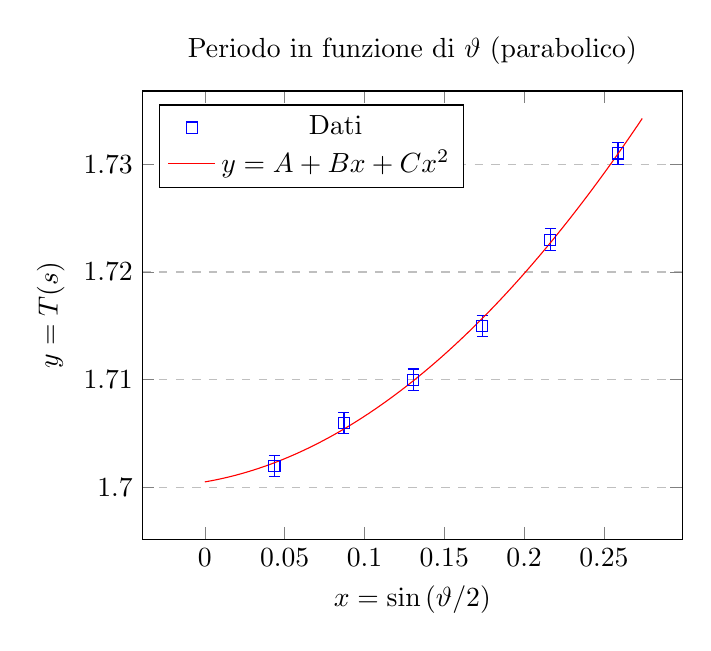
\begin{tikzpicture}
				\begin{axis}[
					title={Periodo in funzione di $\vartheta$ (parabolico)},
					ylabel={$y = T(s)$},
					xlabel={$x = \sin{\left( \vartheta / 2\right) }$},
					xmin=0, xmax=0.26,
					ymin=1.700, ymax=1.732,
					xtick={},
					ytick={},
					tick label style={/pgf/number format/fixed},
					legend pos=north west,
					ymajorgrids=true,
					grid style=dashed,
					enlargelimits=0.15,
					]
					
					\addplot[
					only marks,
					mark=square,
					color=blue,
					error bars/.cd,
					y dir=both, y explicit
					]
					coordinates {
						(0.0436194,1.702) +- (0,0.001)
						(0.0871557,1.706) +- (0,0.001)
						(0.1305262,1.710) +- (0,0.001)
						(0.1736482,1.715) +- (0,0.001)
						(0.2164396,1.723) +- (0,0.001)
						(0.2588190,1.731) +- (0,0.001)
					};
					\addplot[
					domain=0:0.274, 
					samples=100, 
					color=red, 
					] 
					{0.35725602*x^2 + 0.0252062*x + 1.700522};
					\legend{Dati,$y=A+Bx+Cx^2$}
				\end{axis}
			\end{tikzpicture}
		\end{figure}
	\end{minipage}
	\begin{minipage}{0.3\textwidth}
		\begin{table}[H]
			\centering
			\begin{tabular}{@{}rr@{}}
				 $\sin{\left(\vartheta/2\right)}$ & $T(s) \pm 0.001$ \\ \midrule
				0.044&  1.702  \\
				0.087&  1.706  \\
				0.130& 1.710   \\
				0.174& 1.715   \\
				0.216&  1.723  \\
				0.259&  1.731  \\	\bottomrule
			\end{tabular}
		\end{table}	
		\[
		\mathbf{A} = 1.700 \text{ (s)}\qquad \mathbf{\sigma_A} = 0.002 \text{ (s)}
		\]
		\[ 
		\mathbf{B} = 0.025  \text{ (s)}\qquad \mathbf{\sigma_B} = 0.027 \text{ (s)}
		\]
		\[
		\mathbf{C} = 0.357 \text{ (s)} \qquad \mathbf{\sigma_C} = 0.088 \text{ (s)}
		\]
	\end{minipage}
	\vspace{0.8cm}
	
	
	\subsubsection{Test del chi quadro}
	Assumendo che la parabola trovata $y=A+Bx+Cx^2$ si adatti bene all'andamento dei dati scelgo un livello di significatività $\alpha = 0.05$ ed eseguo il test.
	
	\paragraph{Ipotesi nulla} La parabola con parametri \textbf{A},\textbf{B} e \textbf{C} si adatta bene all'andamento dei miei dati.
	
	\vspace{0.7cm}
	\begin{table}[H]
		\centering
		\rowcolors{1}{gray!25}{white}
		\begin{tabular}{lr} 
			Livello di significatività $\alpha$		&$\quad 0.05$  \\
			Valore di $\chi ^2$             		& $\quad 0.96$       \\
			Numero di gradi di libertà      		& $\quad (6-3) = 3$         \\   
			Valore di $\chi ^2$ sospetto			& $\quad 0.35$ \\
			Valore di $\chi ^2$ critico     		& $\quad 7.81$
		\end{tabular}
	\end{table}
	\vspace{0.7cm}
	
	\paragraph{Conclusione test}
	Il valore del chi quadro calcolato risulta essere compreso tra il valore sospetto e quello critico: $\chi^2_\text{sospetto} < \chi ^2 < \chi^2_\text{critico}$ posso quindi affermare che, con livello di significatività del 5\%, la parabola descritta dai parametri \textbf{A},\textbf{B} e \textbf{C} si adatta bene all'andamento dei miei dati.
	
	
	\subsubsection{Test Z}
	Constatato che la parabola descrive bene l'andamento dei miei dati vado a confrontare i parametri ottenuti con quelli teorici per capire se questi siano compatibili. La parabola  teorica
	\[
	T = T_0 + \frac{T_0}{4}\sin{(\vartheta/2)}^2
	\]
	ha come parametri 
	\[
	A_\text{teo} = T_0 \qquad B_\text{teo} = 0 \qquad C_\text{teo} =  \frac{T_0}{4} 
	\]
	
	\noindent
	Procedo quindi con un Test Z per verificare la compatibilità tra i valori:
	
	\paragraph{Ipotesi nulla} I parametri della parabola sperimentale sono compatibili con i parametri della parabola teorica.
	
	\vspace{0.7cm}
	\begin{minipage}{0.5\textwidth}
		\begin{table}[H]
			\centering
			\rowcolors{1}{gray!25}{white}
			\begin{tabular}{lr} 
				Livello di significatività $\alpha$		&$\quad 0.05$  \\
				\textbf{A} sperimentale				& $\quad1.700 \pm 0.002 $\\
				\textbf{A} teorico					& $\quad T_0  = 1.704 \pm 0.002$ \\
				$z_{A}$ osservato 					& $\quad$1.08 \\
				$z$ critico     	& $\quad 1.96$
			\end{tabular}
		\end{table}
	\end{minipage}
	\begin{minipage}{0.5\textwidth}
		\begin{table}[H]
			\centering
			\rowcolors{1}{gray!25}{white}
			\begin{tabular}{lr} 
				Livello di significatività $\alpha$		&$\quad 0.05$  \\
				\textbf{B} sperimentale				& $\quad0.025 \pm  0.027$	\\ 
				\textbf{B} teorico					& $\quad 0$ \\
				$z_{B}$ osservato 					& $\quad$ 0.92 \\
				$z$ critico     	& $\quad 1.96$
			\end{tabular}
		\end{table}
	\end{minipage}
	
	\begin{table}[H]
		\centering
		\rowcolors{1}{gray!25}{white}
		\begin{tabular}{lr} 
			Livello di significatività $\alpha$		&$\quad 0.05$  \\
			\textbf{C} sperimentale             	& $\quad0.357 \pm 0.088$     \\
			\textbf{C} teorico					&  $\quad T_0/4 = 0.425 \pm 0.005$\\
			$z_{C}$ osservato					& 0.78 \\ 
			$z$ critico     	& $\quad 1.96$
		\end{tabular}
	\end{table}
	\footnote{Poiché anche il valore di $T_0$ ha una sua incertezza (dipende dalla lunghezza misurata da me) il valore di $z_A$ osservato è calcolato come $z_A = \frac{|A_{\text{teo} - A_{\text{sper}}}|}{\sqrt{\sigma_A^2 + \sigma_{T_0}^2}}$ dove $\sigma_{T_0} = \frac{\partial}{\partial l}\left(2\pi\sqrt{\frac{l}{g}}\right)\sigma_l =  \frac{\pi}{\sqrt{gl}} \sigma_l $. 
	
	Stessa cosa per $z_C$ che è stato calcolato nello stesso modo ma con $\sigma_{T_0/4} = \frac{\pi}{4\sqrt{gl}} \sigma_l$. \\
	
	\noindent
	Inoltre per i valori di A,B e C sia sperimentali sia teorici scelgo di lasciare 3 cifre decimali per poter scrivere anche gli errori associati più piccoli.}
	\vspace{0.7cm}
	
	\paragraph{Conclusione test}
	Poiché ogni $z_\text{oss}$ risulta minore dello $z_\text{critico}$,  concludo che, con un livello di significatività del 5\%, tutti i parametri risultano essere compatibili con le aspettative teoriche.
	
	%%%%%%%%%%%%%%%%%%%%%%%%%%%%%%%%%%%%%%%%%%%%%%%%%%%%%%%%%
	%%				DIPENDENZA ELLE     LLLLL
	%%%%%%%%%%%%%%%%%%%%%%%%%%%%%%%%%%%%%%%%%%%%%%%%%%%%%%%%%
	
	\newpage
	\section{Dipendenza dalla lunghezza}
	La seconda parte dell'esperienza consiste nel verificare la dipendenza del periodo di oscillazione del pendolo dalla sua lunghezza. Nell'equazione che descrive il periodo $l$ compare sotto radice quindi, per studiarne la relazione lineare si eleva tutto al quadrato così da avere $T^2$ in funzione di $l$:
	
	\[
	T = 2\pi \sqrt{\frac{l}{g}} \left( 1 + \frac{1}{4}\sin{\left(\vartheta/2\right)}^2 \right) \qquad T^2 = 4 \pi^2 \frac{l}{g} \left( 1 + \frac{1}{4}\sin{\left(\vartheta/2\right)}^2 \right)^2
	\]
	\[
	T^2 = C_3 l
	\]
	con $C_3 =  \frac{4 \pi^2}{g} \left( 1 + \frac{1}{4}\sin{\left(\vartheta/2\right)}^2 \right)^2$ \\
	
	\subsection{Acquisizione dati}
	Per prima cosa procedo con le misurazioni di 5 pendoli di 5 diverse lunghezze. Con l'ausilio dell'asta graduata, come fatto in precedenza, misuro prima la distanza da terra alla cima del pendolo ($L_C$) e poi la distanza da terra al centro della sfera appesa ($L_F$). Come errore su $l$ associo 2 volte la sensibilità dell'asta. Appesa al filo del pendolo c'è una sfera di massa $m = (110 \pm 1)g$.
	\[
	l_i =( L_C - L_{F_i}  \pm 0.2) \text{cm}\qquad i= 1, \dots, 5
	\]
	
	\begin{table}[H]
		\centering
		\begin{tabular}{@{}ccccc@{}}
			$\mathbf{l_1}$ & $\mathbf{l_2}$ & $\mathbf{l_3}$ & $\mathbf{l_4}$ & $\mathbf{l_5}$  \\ \midrule
			$l_1(\text{cm}) \pm 0.2\text{cm}$  & $l_2(\text{cm}) \pm 0.2\text{cm}$  & $l_3(\text{cm}) \pm 0.2\text{cm}$ & $l_4(\text{cm}) \pm 0.2\text{cm}$ & $l_5(\text{cm}) \pm 0.2\text{cm}$\\ \midrule
			\multicolumn{1}{r}{57.2} & \multicolumn{1}{r}{23.7} & \multicolumn{1}{r}{13.5} & \multicolumn{1}{r}{60.0} & \multicolumn{1}{r}{51.8}\\ \bottomrule
		\end{tabular}
	\end{table}
	\vspace{0.5cm}
	
	
	Come per lo studio del periodo in funzione dell'angolo di oscillazione, anche in questo caso registro tre misure del periodo per ogni sua lunghezza con un angolo fisso $\vartheta = 20^\circ \pm 1^\circ$.
	
	\vspace{0.7cm}
	\begin{minipage}{0.1\textwidth}
		\colorbox{blue!40}{$\vartheta = 20^\circ \pm 1^\circ$}
	\end{minipage}
	\begin{minipage}{0.1\textwidth}
	\begin{table}[H]
		\centering
		\begin{tabular}{@{}lrrrrr@{}}
			& $\mathbf{l_1}$ & $\mathbf{l_2}$ & $\mathbf{l_3}$ & $\mathbf{l_4}$ & $\mathbf{l_5}$  \\ \cmidrule(l){2-6}   
			& $T(s) \pm 0.001s$ & $T(s) \pm 0.001s$   & $T(s) \pm 0.001s$ & $T(s) \pm 0.001s$ & $T(s) \pm 0.001s$  \\ \cmidrule(l){2-6} 
			
			\multicolumn{1}{c}{}  
			
			 & 1.504 & 0.964 & 0.663 & 1.556 & 1.437 \\
			& 1.504 & 0.962 & 0.662 & 1.558 & 1.437 \\
			& 1.502 & 0.962 & 0.663 & 1.555 & 1.436 \\
			
			\arrayrulecolor{black!100}\specialrule{1.2pt}{0.5\jot}{0.5pc}
			
			$\mathbf{\bar{T}(s)}$ & \textbf{1.503} & \textbf{0.9627} & \textbf{0.6627} & \textbf{1.556} & \textbf{1.437}     
		\end{tabular}
	\end{table}
	\end{minipage}
	
	
	
	
	\vspace{1cm}
		
	\subsection{Retta di best-fit}
	Per applicare al meglio il metodo dei minimi quadrati controllo quale delle due variabili ha errore relativo più piccolo.
	
	\begin{minipage}{0.5\textwidth}
		\begin{table}[H]
			\centering
			\begin{tabular}{@{}ccc@{}}
				\multicolumn{3}{c}{$\mathbf{T^2}$} \\ \midrule
				$T^2(s)$ & $\sigma_{T^2} (s)$ & $\sigma_{T^2} / T^2$ \\ \midrule
				2.26 & 0.003 & \textbf{0.0013 }\\
				0.926 & 0.002 & \textbf{0.0021} \\
				0.439 & 0.001 & \textbf{0.0030} \\
				2.422 & 0.003 & \textbf{0.0013} \\
				2.064 & 0.003 & \textbf{0.0014}  \\ \bottomrule   
			\end{tabular}
		\end{table}
	\end{minipage}
	\begin{minipage}{0.5\textwidth}
		\begin{table}[H]
			\centering
			\begin{tabular}{@{}ccc@{}}
				\multicolumn{3}{c}{\textbf{l}} \\ \midrule
				$l$(cm) & $\sigma_l$(cm) & $\sigma_l / l$ \\ \midrule
				60.20 & 0.2 & \textbf{0.0033} \\
				26.70 & 0.2 & \textbf{0.0075} \\
				14.50 & 0.2 & \textbf{0.0138} \\
				63.00 & 0.2 & \textbf{0.0032} \\
				54.80 & 0.2 & \textbf{0.0036} \\ \bottomrule  
			\end{tabular}
		\end{table}
	\end{minipage}
	\vspace{1cm}
	
	\noindent
	L'errore associato a $l$ risulta essere significativamente più grande di quello su $T^2$ quindi decido di invertire la relazione per poter mettere sull'asse $x$ il periodo al quadrato:
	\[
	l = \frac{1}{C_3} T^2
	\]
	
	
	\begin{minipage}{0.3\textwidth}
		\begin{table}[H]
			\centering
			\begin{tabular}{@{}ll@{}}
				$T^2(s)$ & \multicolumn{1}{l}{$(l \pm 0.2)$cm} \\ \midrule
				2.26&57.2     \\
				0.93&23.7    \\
				0.44&11.4   \\
				2.42&60.0    \\
				2.06&51.8   \\	\bottomrule
			\end{tabular}
		\end{table}	
		\[
		\mathbf{A} = 0.7 \text{ (cm)}  \qquad \mathbf{\sigma_A} = 0.3 \text{ (cm)}
		\]
		\[
		\mathbf{B} = 24.7 \text{ (cm}/s^2) \qquad \mathbf{\sigma_B} = 0.1 \text{ (cm}/s^2)
		\]
	\end{minipage}
	\begin{minipage}{0.3\textwidth}
		\begin{figure}[H]
			\hspace{1cm}
			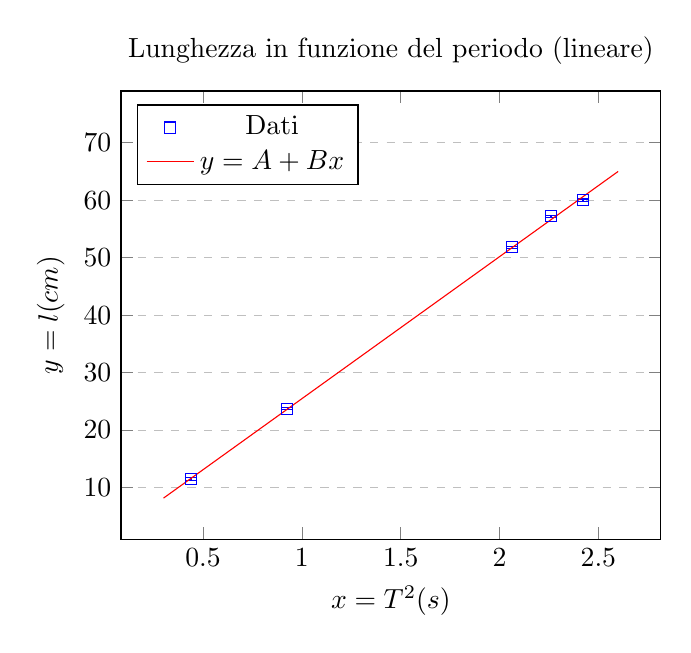
\begin{tikzpicture}
				\begin{axis}[
					title={Lunghezza in funzione del periodo (lineare)},
					xlabel={$x = T^2(s)$},
					ylabel={$y = l(cm)$},
					xmin=0.4, xmax=2.5,
					ymin=10, ymax=70,
					xtick={0,0.5,1,1.5,2,2.5},
					ytick={0,10,20,30,40,50,60,70},
					legend pos=north west,
					ymajorgrids=true,
					grid style=dashed,
					enlargelimits=0.15,
					]
					
					\addplot[
					only marks,
					color=blue,
					mark=square,
					error bars/.cd,
					y dir=both, y explicit
					]
					coordinates {
						(2.260011111,57.20) +- (0,0.2)
						(0.9267271111,23.70) +- (0,0.2)
						(0.4391271111,11.50) +- (0,0.2)
						(2.422173444,60.00) +- (0,0.2)
						(2.064011111,51.80) +- (0,0.2)
					};
					\addplot[
					domain=0.3:2.6, 
					samples=100, 
					color=red, 
					] 
					{ 24.7131*x + 0.7451};
					\legend{Dati,$y=A + Bx$}
				\end{axis}
			\end{tikzpicture}
		\end{figure}
	\end{minipage}
	
	
	\subsubsection{Test del chi quadro}
	Visti i risultati ottenuti assumo che la retta trovata di parametri $\mathbf{A}$ e $\mathbf{B}$ si adatti bene all'andamento dei miei dati. Per assicurarmene effettuo un test del $\chi^2$
	
	\paragraph{Ipotesi nulla} La retta $y = A + Bx$ descrive bene l'andamento dei dati osservati sperimentalmente.
	
	\vspace{0.7cm}
	\begin{table}[H]
		\centering
		\rowcolors{1}{gray!25}{white}
		\begin{tabular}{lr} 
			Livello di significatività $\alpha$		&$\quad 0.05$  \\
			Valore di $\chi ^2$             	& $\quad 18.58$       \\
			Numero di gradi di libertà      	& $\quad (5-2) = 3$         \\   
			Valore di $\chi ^2$ critico     	& $\quad 7.81$
		\end{tabular}
	\end{table}
	\vspace{0.7cm}
	
	\paragraph{Conclusione test} Il valore del $\chi^2$ ottenuto risulta essere maggiore del valore critico, rifiuto quindi l'ipotesi nulla. Un valore di chi quadro così elevato mi porta a credere che la dispersione dei miei dati attorno alla retta sia troppo elevata e probabilmente di aver sottostimato l'errore su $l$. 
	
	Poiché il coefficiente di correlazione lineare $r = 0.9998 \approx 1$ evidenzia (e conferma) la relazione di linearità tra $l$ e $T^2$, decido di calcolare l'errore $\sigma_y'$ a  posteriori così da determinare l'incertezza corretta delle $y$.
	\[
	\text{errore a posteriori: } \sigma_y' = 0.49
	\]	
	Con il nuovo valore dell'incertezza delle $y$ posso ricalcolare i parametri della retta con una maggiore affidabilità e rigraficare il tutto:
	
	\begin{minipage}{0.3\textwidth}
		\begin{table}[H]
			\centering
			\begin{tabular}{@{}ll@{}}
				$T^2(s) \pm \sigma_{T^2}$ & \multicolumn{1}{l}{$(l \pm 0.5)$cm} \\ \midrule
				2.26&57.2    \\
				0.93&23.7    \\
				0.44&11.4    \\
				2.42&60.0    \\
				2.06&51.8    \\	\bottomrule
			\end{tabular}
		\end{table}	
		\[
		\mathbf{A'} = 0.7 \text{ (cm)} \qquad \mathbf{\sigma_{A'}} = 0.5 \text{ (cm)} 
		\]
		\[
		\mathbf{B'} = 24.7 \text{ (cm}/s^2) \qquad \mathbf{\sigma_{B'}} = 0.3 \text{ (cm}/s^2)
		\]
	\end{minipage}
	\begin{minipage}{0.3\textwidth}
		\begin{figure}[H]
			\hspace{1cm}
			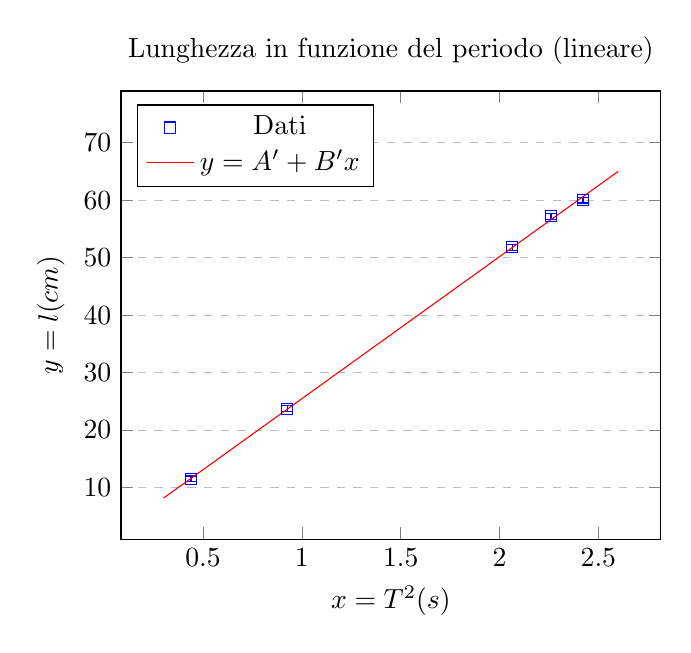
\begin{tikzpicture}
				\begin{axis}[
					title={Lunghezza in funzione del periodo (lineare)},
					xlabel={$x = T^2(s)$},
					ylabel={$y = l(cm)$},
					xmin=0.4, xmax=2.5,
					ymin=10, ymax=70,
					xtick={0,0.5,1,1.5,2,2.5},
					ytick={0,10,20,30,40,50,60,70},
					legend pos=north west,
					ymajorgrids=true,
					grid style=dashed,
					enlargelimits=0.15,
					]
					\addplot[
					only marks,
					color=blue,
					mark=square,
					error bars/.cd,
					y dir=both, y explicit
					]
					coordinates {
						(2.260011111,57.20) +- (0,0.4978)
						(0.9267271111,23.70) +- (0,0.4978)
						(0.4391271111,11.50) +- (0,0.4978)
						(2.422173444,60.00) +- (0,0.4978)
						(2.064011111,51.80) +- (0,0.4978)
					};
					\addplot[
					domain=0.3:2.6, 
					samples=100, 
					color=red, 
					] 
					{ 24.7131*x + 0.7451};
					\legend{Dati,$y=A' + B'x$};
				\end{axis}
			\end{tikzpicture}
		\end{figure}
	\end{minipage}
	
	
	\subsubsection{Test Z}
	Dal test del chi quadro ho appurato che la retta $y = A + Bx$ non è una buona rappresentazione dell'andamento dei miei dati. Scegliendo l'errore a posteriori come errore associato ai valori sulle y trovo una retta meglio rappresentativa. Mi interessa allora capire se l'andamento teorico si adatta bene alla retta $y = A' + B'x$, ovvero se l'equazione teorica
	\[
	l = \frac{1}{C_3} T^2 \qquad \text{con } C_3 =  \frac{4 \pi^2}{g} \left( 1 + \frac{1}{4}\sin{\left(\vartheta/2\right)}^2 \right)^2
	\]
	che ha come parametri
	\[
	A_\text{teo} = 0 \qquad B_\text{teo} =  \frac{1}{C_3}
	\]
	si adatta bene alla retta. 
	
	\paragraph{Ipotesi nulla} I valori $A_{\text{teo}}$, $\mathbf{A}$ e  $B_{\text{teo}}$, $\mathbf{B}$ sono a due a due compatibili.
	
	\vspace{0.7cm}
	\begin{minipage}{0.5\textwidth}
		\begin{table}[H]
			\centering
			\rowcolors{1}{gray!25}{white}
			\begin{tabular}{lr} 
				Livello di significatività $\alpha$		&$\quad 0.05$  \\
				\textbf{A'} sperimentale				& $\quad0.7 \pm 0.5 $\\
				\textbf{A'} teorico					&  $\quad0$ \\
				$z_{A'}$ osservato 					& $\quad$ 1.47 \\
				Valore di $Z$ critico     	& $\quad 1.96$
			\end{tabular}
		\end{table}
	\end{minipage}
	\begin{minipage}{0.5\textwidth}
		\begin{table}[H]
			\centering
			\rowcolors{1}{gray!25}{white}
			\begin{tabular}{lr} 
				Livello di significatività $\alpha$		&$ 0.05$  \\
				\textbf{B'} sperimentale				& $ 24.7 \pm  0.3$	\\
				\textbf{B'} teorico					& $ 1/C_3 = 24.5 \pm 0.04$ \footnotemark \\
				$z_{B'}$ osservato 					&  0.83 \\
				Valore di $Z$ critico     	& $ 1.96$
			\end{tabular}
		\end{table}
	\end{minipage}
	\vspace{0.7cm}
	
	
	\footnotetext{Poiché anche il valore di $1/C_3$ ha una sua incertezza (dipende dall'angolo misurato) il valore di $z_{B'}$ osservato è calcolato come $z_A = \frac{|B'_{\text{teo}} - B'_{\text{sper}}|}{\sqrt{\sigma_B^2 + \sigma_{1/C_3}^2}}$ dove $\sigma_{1/C_3} = \frac{\partial}{\partial \vartheta}\left[ \frac{4 \pi^2}{g} \left( 1 + \frac{1}{4}\sin{\left(\vartheta/2\right)}^2 \right)^2  \right] = \frac{g\sin{(\vartheta)}}{16\pi^2\left(1 + \frac{sin^2{(\vartheta/2)}}{4}\right)^3} \sigma_\vartheta$.}
	\paragraph{Conclusione test} Poiché sia per $\mathbf{A'}$ sia per $\mathbf{B'}$ risulta che $z_{\text{oss}}$ < $z_{\text{critico}}$ posso affermare che ognuno dei parametri  è compatibile con il rispettivo valore teorico nei livelli di significatività scelti e che quindi l'equazione teorica della retta è una buona rappresentazione della retta $y=A' + B'x$.\\
	
	
	
	
	
	
	%%%%%%%%%%%%%%%%%%%%%%%%%%%%%%%%%%%%%%%%%%%%%%%%%%%%%%%%%
	%%				DIPENDENZA MASSA     MMMM
	%%%%%%%%%%%%%%%%%%%%%%%%%%%%%%%%%%%%%%%%%%%%%%%%%%%%%%%%%
	
	\section{Dipendenza dalla massa}
	Come si può osservare dall'equazione del periodo, questo non è teoricamente influenzato dalla massa appesa ad esso. Tuttavia, sperimentalmente, la massa potrebbe portare a delle più o meno lievi variazioni. A seconda della massa in esame infatti, potrebbe variare la lunghezza del filo che viene allungato dal peso del corpo, oppure per masse estremente piccole non sarebbe più ragionevole pensare che la massa del filo sia trascurabile.
	
	
	
	\subsection{Acquisizione dati}
	Prese 3 sfere (una vuota, una piena d'acqua e una piena di piombo) di uguale volume, ne registro la massa pesandole con una bilancia. Agganciate al pendolo misuro l'allungamento di quest'ultimo dovuto al peso delle sfere. La lunghezza del pendolo è stata misurata con l'asta graduata mentre l'allungamento, essendo nell'ordine dei millimetri, con un calibro. 
	
	A seguito delle misure ottengo le seguenti masse con le rispettive lunghezze del filo:
	
	\vspace{0.5cm}
	\begin{table}[H]
		\centering
		\begin{tabular}{@{}lcc@{}}
				& \multicolumn{1}{l}{$m(\text{g}) \pm 1$g} & \multicolumn{1}{l}{$L(\text{cm}) \pm 0.2$cm}  \\ \midrule
			$m_1$ (vuota)   & 9& 63.90                                            \\
			$m_2$ (acqua)  & 108 & 64.00                                          \\
			$m_3$ (piombo)  & 647  & 64.60                                        \\ \bottomrule
		\end{tabular}
	\end{table}
	\vspace{0.5cm}
	
	Con un angolo di oscillazione fisso di $20^\circ$ prendo 3 misure del periodo per ogni massa ottenendo i seguenti dati:
	
	\vspace{0.7cm}
	\begin{minipage}{0.2\textwidth}
		\colorbox{blue!40}{$\vartheta = 20^\circ \pm 1^\circ$}
	\end{minipage}
	\begin{minipage}{0.4\textwidth}
	\begin{table}[H]
		\centering
		\begin{tabular}{@{}lrrr@{}}
			& $\mathbf{m_1}$ \textbf{(vuota)} & $\mathbf{m_2}$ \textbf{(acqua)} & $\mathbf{m_3}$ (\textbf{piombo})   \\ \cmidrule(l){2-4}   
			& $T(s) \pm 0.001s$ & $T(s) \pm 0.001s$   & $T(s) \pm 0.001s$  \\ \cmidrule(l){2-4} 
			
			\multicolumn{1}{c}{}  
			
			&1.675 & 1.689 & 1.694  \\
			&1.671 & 1.689 & 1.694  \\
			&1.670 & 1.689 & 1.695 \\
			
			\arrayrulecolor{black!100}\specialrule{1.2pt}{0.5\jot}{0.5pc}
			
			$\mathbf{\bar{T}(s)}$ & \textbf{1.672}    & \textbf{1.689}  & \textbf{1.694}        
		\end{tabular}
	\end{table}
	\end{minipage}
	\vspace{0.5cm}
	
	\subsection{Test Z}
	Per capire se i periodi ottenuti con le tre sfere sono compatibili confronto le loro differenze con zero. Eseguo quindi tre test Z.
	
	\paragraph{Ipotesi nulla} I periodi di oscillazione del pendolo con massa $m_1$, $m_2$ e $m_3$ sono a due a due compatibili.
	
		\vspace{0.7cm}
	\begin{minipage}{0.5\textwidth}
		\begin{table}[H]
			\centering
			\rowcolors{1}{gray!25}{white}
			\begin{tabular}{lr} 
				Livello di significatività $\alpha$		&$\quad 0.05$  \\
				$z_{T_{1,2}}$ osservato 					& $\quad$ 6.15 \\
				Valore di $Z$ critico     	& $\quad 1.96$
			\end{tabular}
		\end{table}
	\end{minipage}
	\begin{minipage}{0.5\textwidth}
		\begin{table}[H]
			\centering
			\rowcolors{1}{gray!25}{white}
			\begin{tabular}{lr} 
				Livello di significatività $\alpha$		&$\quad 0.05$  \\
				$z_{T_{2,3}}$ osservato 					& $\quad$ 8.20 \\
				Valore di $Z$ critico     	& $\quad 1.96$
			\end{tabular}
		\end{table}
	\end{minipage}
	\begin{table}[H]
		\centering
		\rowcolors{1}{gray!25}{white}
		\begin{tabular}{lr} 
			Livello di significatività $\alpha$		&$\quad 0.05$  \\
			$z_{T_{1,3}}$ osservato 					& $\quad$ 2.05 \\
			Valore di $Z$ critico     	& $\quad 1.96$
		\end{tabular}
	\end{table}
	
	\paragraph{Conclusione test} Poiché ogni $z$ osservato risulta maggiore dello $z$ critico rigetto l'ipotesi nulla e concludo affermando che nessun periodo misrato è compatibile con una massa differente. Nonostante questo sembra contraddire la teoria, ritengo che l'esito dei test sia concorde con le aspettative sperimentali; si sono infatti osservati cambiamenti nella lunghezza del pendolo per ogni massa appesa ad esso, il che rende coerenti le discrepanze tra i periodi misurati.
	
	%%%%%%%%%%%%%%%%%%%%%%%%%%%%%%%%%%%%%%%%%%%%%%%%%%%%%%%%%
	%%				    CONCLUSIONI
	%%%%%%%%%%%%%%%%%%%%%%%%%%%%%%%%%%%%%%%%%%%%%%%%%%%%%%%%%
	
	\section{Conclusioni}
	L'esperienza di laboratorio aveva come obiettivo lo studio del periodo di oscillazione del pendolo semplice al variare dell'angolo di partenza, della sua lunghezza e della massa appesa ad esso. Al fine di eseguire delle misure del periodo precise ho testato tre strumenti di misura differenti: un cronometro digitale, uno analogico e una fotocellula. Ho quindi acquisito 8 periodi con un angolo di partenza di $5^\circ \pm 1^\circ$ e altri 8 con un'angolo di $30^\circ \pm 1^\circ$ con ciascuno strumento. A seguito di un test Z si è constatato che i due cronometri fornivano periodi compatibili (con un livello di significatività maggiore dell'80\%) per i due angoli di partenza. La fotocellula invece registrava periodi significativamente distinguibili per ciascun angolo; per questo ho deciso di utilizzare la fotocellula come strumento per le successive acquisizioni di dati.
	
	\paragraph{T(0) Dipendenza dall'angolo}
	Al fine di studiare la dipendenza di $T$ da $\vartheta$ ho acquisito tre periodi di oscillazione per 6 angoli differenti per poi andare a studiare la relazione lineare tra $T$ e $\sin^2(\vartheta/2)$ e parabolica tra $T$ e $\sin(\vartheta/2)$ come vuole la teoria.
	
	Tramite il metodo dei minimi quadrati ho ricavato i parametri della retta e della parabola e con un test del chi quadro ho verificato che le curve descrivessero bene l'andamento dei dati sperimentali, ottenendo in entrambi i casi esiti positivi con livello di significatività del 5\%. Ho poi verificato che le curve teoriche si adattassero bene a quelle sperimentali sottoponendo a un test Z i parametri di retta e parabola; anche in questo caso andamento teorico e sperimentale sono risultati compatibili con un livello di significatività del 5\%.
	
	Infine ho ricavato il valore di $g$ accelerazione di gravità a partire dai dati sperimentali ottenendo 	$g = (830 \pm 81)\text{cm}\cdot \text{s}^{-2}$. Sottoposto quest'utltomo a un test Z ho constatato che risulta compatibile,  con un livello di significatività del 5\%, con il valore vero $G = 981\text{cm}\cdot \text{s}^{-2}$.
	
	\paragraph{T(l) Dipendenza dalla lunghezza}	
	Per evidenziare la dipendenza di $T$ da $l$ ho studiato la linearità tra $T^2$ e $l$ ($l$ compare sotto radice). Ho quindi acquisito tre periodi per 5 diverse lunghezze e sempre con il metodo dei minimi quadrati ho ricavato i parametri della retta di best-fit. 
	
	Un primo test del chi quadro ha evidenziato una sottostima degli errori su $l$, ho quindi deciso di associare l'errore a posteriori come incertezza di $l$ ricavando una seconda retta. Un secondo test del chi quadro e un test Z hanno confermato la compatibiltà tra l'andamento dei miei dati e la retta e tra questa e l'andamento teorico (entrambi con un livello di significatività del 5\%).
	
	\paragraph{T(m) Dipendenza dalla massa}
	Infine ho studiato la dipendenza dalla massa di $T$. Seppure questo non sia teoricamente dipendente da essa, le misurazioni acquisite con 3 masse differenti hanno evidenziato delle variazioni significative del periodo. Andando a sottoporre 3 periodi differenti misurati con 3 sfere con masse diverse ad un test Z, con un livello di significatività del 5\%, nessuno di questi è risultato comopatibile con uno degli altri.
	
	I risultati del test sono comprensibili e imputabili all'allungamento del filo causato dalle masse.
	
	
\end{document}